\section{Introduction}
Variation in human color preferences across cultures and sexes has not been well characterized. The majority of past studies have worked with relatively small samples of participants asked to make explicit decisions with limited stimuli consisting of blocks of single colors. 
Using this method, Hurlbert and Ling ~\cite{hurlbert2007biological} found a universal preference for bluish hues, along with a greater cross-cultural female preference for reddish hues.
They gave an evolutionary explanation related to the adaptive benefit to foraging females of seeking out a red object on a green background (e.g., fruit against leaves).  
Palmer and Schloss ~\cite{palmer2010ecological} argued that color preferences can be explained in terms of object preferences and associations between objects and colors, which can be influenced by evolution, culture, and individual experience.  The question of sex differences was left open in this paper.

We propose that large-scale novel data-mining of images available on the Web can overcome the limitation of study sizes. Moreover, the metadata associated with the web-scale images provides more interesting information for our complimentary studies.
When people upload their photos to social networks, they are sharing information about which scenes and types of photos they prefer.
By analyzing the color spectra over 15 million photographs on Flickr, an online photo-sharing network, we measure male and female preferences in an implicit (behavior-based) rather than explicit (ratings-based) manner and on a much larger scale than can be done in a lab experiment.
We find strong sex differences for the predominant reddish and bluish hues, with female users uploading more photographs containing more reddish pixels and male users uploading more photographs containing more bluish pixels.
To take a step towards exploring the reason for this difference and the relation of content preference and color preference, we analyze the least entropy textual tags used by photographers taking photos with most amount of color pixels in each hue interval. Furthermore, we take Google Street View to represent the color distribution in the environment, and compare with Flickr photos in three popular outdoor locations. We study the color distribution and observe the overall preference of saturated color and reddish color of human compared to the environment.

\section{Differences in Color Distributions on Flickr}
To characterize each photo's color distribution, we consider color histograms in CIE L*C*h* (LCh) color space representing each pixel in a perceptually-uniform space according to Lightness, Chroma, and Hue dimensions.
Here we focus only on the Hue dimension, dividing it evenly into 65 discrete bins.
Each photo is first converted into a histogram of the distribution of pixels over hue angle. We then normalize the histogram by user, and take the histograms of all users from a particular population (e.g., men) and combine them into a single aggregated histogram.

We first analyze a general dataset with a larger number of images and without any constraint on content, photographer or location where the photos are taken.
We collected data for about 150 million publicly-available images from Flickr using the public API, as well as public profile information (including gender) for each photographer. We then downloaded a random subset of 15 million photographs taken by 2.8 million photographers.
Preliminary results indicate strong overall sex differences for the predominant reddish and bluish hues, with women uploading more photos with more reddish pixels and men uploading more photos with more bluish pixels (see Fig ~\ref{fig:random}).  

To allow more careful examination of how preferences vary across content and geo-locations, we also downloaded: (1) photos of people uploaded to the Flickr Allpeople group ~\cite{allpeople} 
%~\cite{https://www.flickr.com/groups/allpeople/} 
with at least one human figure on it from 22141 female and 39025 male photographers, and (2) photos geo-tagged within three specific places: Death Valley National Park (with 376 female and 2435 male users), San Diego Balboa Park (with 765 female and 2646 male users), and Disneyland (with 1184 female and 3279 male users).
In Fig ~\ref{fig:allpeople3locations}, we can find the results from all of the four datasets generally support the preliminary results. 
That is, the difference in reddish and bluish color preference between genders is consistent across content and geo-locations.

In addition to directly analyzing the hue distribution of pixels, another experiment presenting in Fig ~\ref{fig:user} also supports our results by examining the distribution of users with ``preference'' of colors along the hue axis.
According to Random dataset, we present the number of users with respect to genders sharing photos with more than $10\%$ pixels in each of the 65 color bins showing the consistent result of gender preference on reddish and bluish color.

\begin{figure}[t]
 \centering
    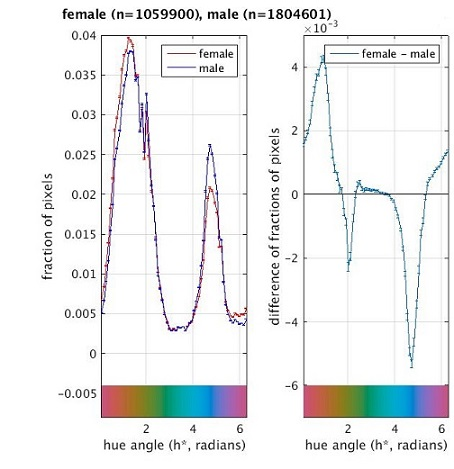
\includegraphics[width=0.489\textwidth]{figures/chapter3/randomhuesmall.jpg}
 \caption{Results on Random dataset. Left: Distribution across hue for male and female photographers. Right: Difference between female and male hue distributions, indicating more reddish hues for women and more bluish hues for men.}
 \label{fig:random}
\end{figure}

\begin{figure*}[th]
\centering
\begin{tabular}{c c}
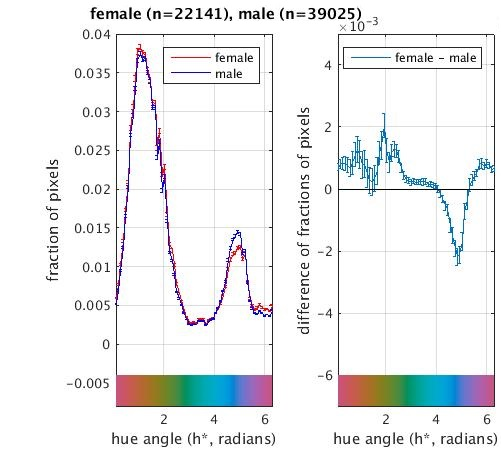
\includegraphics[width=0.45\textwidth]{figures/chapter3/allpeoplehuesmall.jpg} &
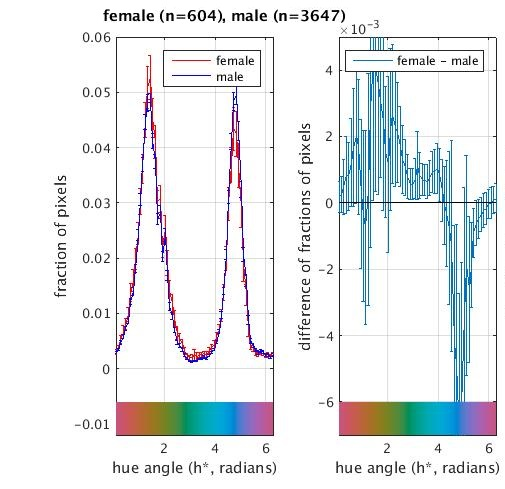
\includegraphics[width=0.45\textwidth]{figures/chapter3/deathvallyhuesmall.jpg} \\
(a) Allpeople dataset&
(b) Death Valley National Park\\
\\
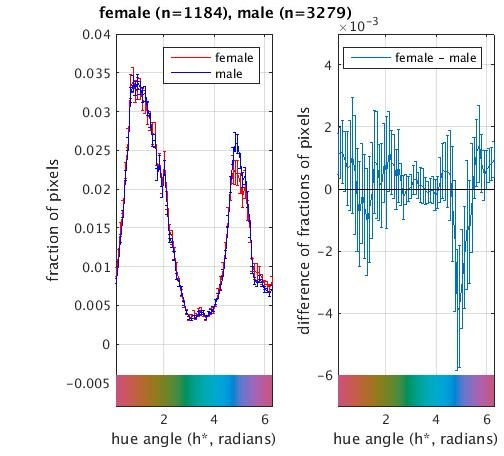
\includegraphics[width=0.45\textwidth]{figures/chapter3/disneyhuesmall.jpg} &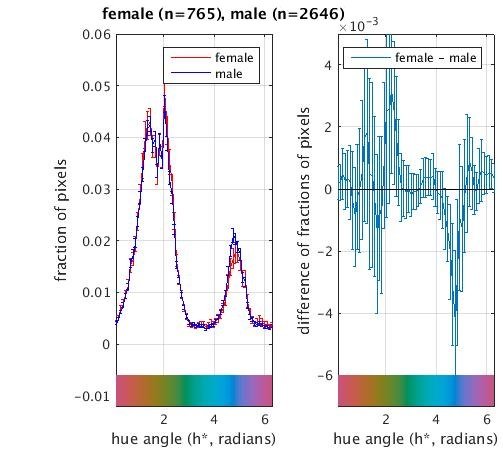
\includegraphics[width=0.45\textwidth]{figures/chapter3/sdzoohuesmall.jpg} \\
(c) Disneyland in Los Angelos&
(d) San Diego Balboa Park\\
\end{tabular}
\caption{Hue distributions and hue difference distributions of 4 different dataset with constraint on content in (a) and locations in (b)-(d).}
\label{fig:allpeople3locations}
\end{figure*}

\begin{figure}[t]
 \centering
    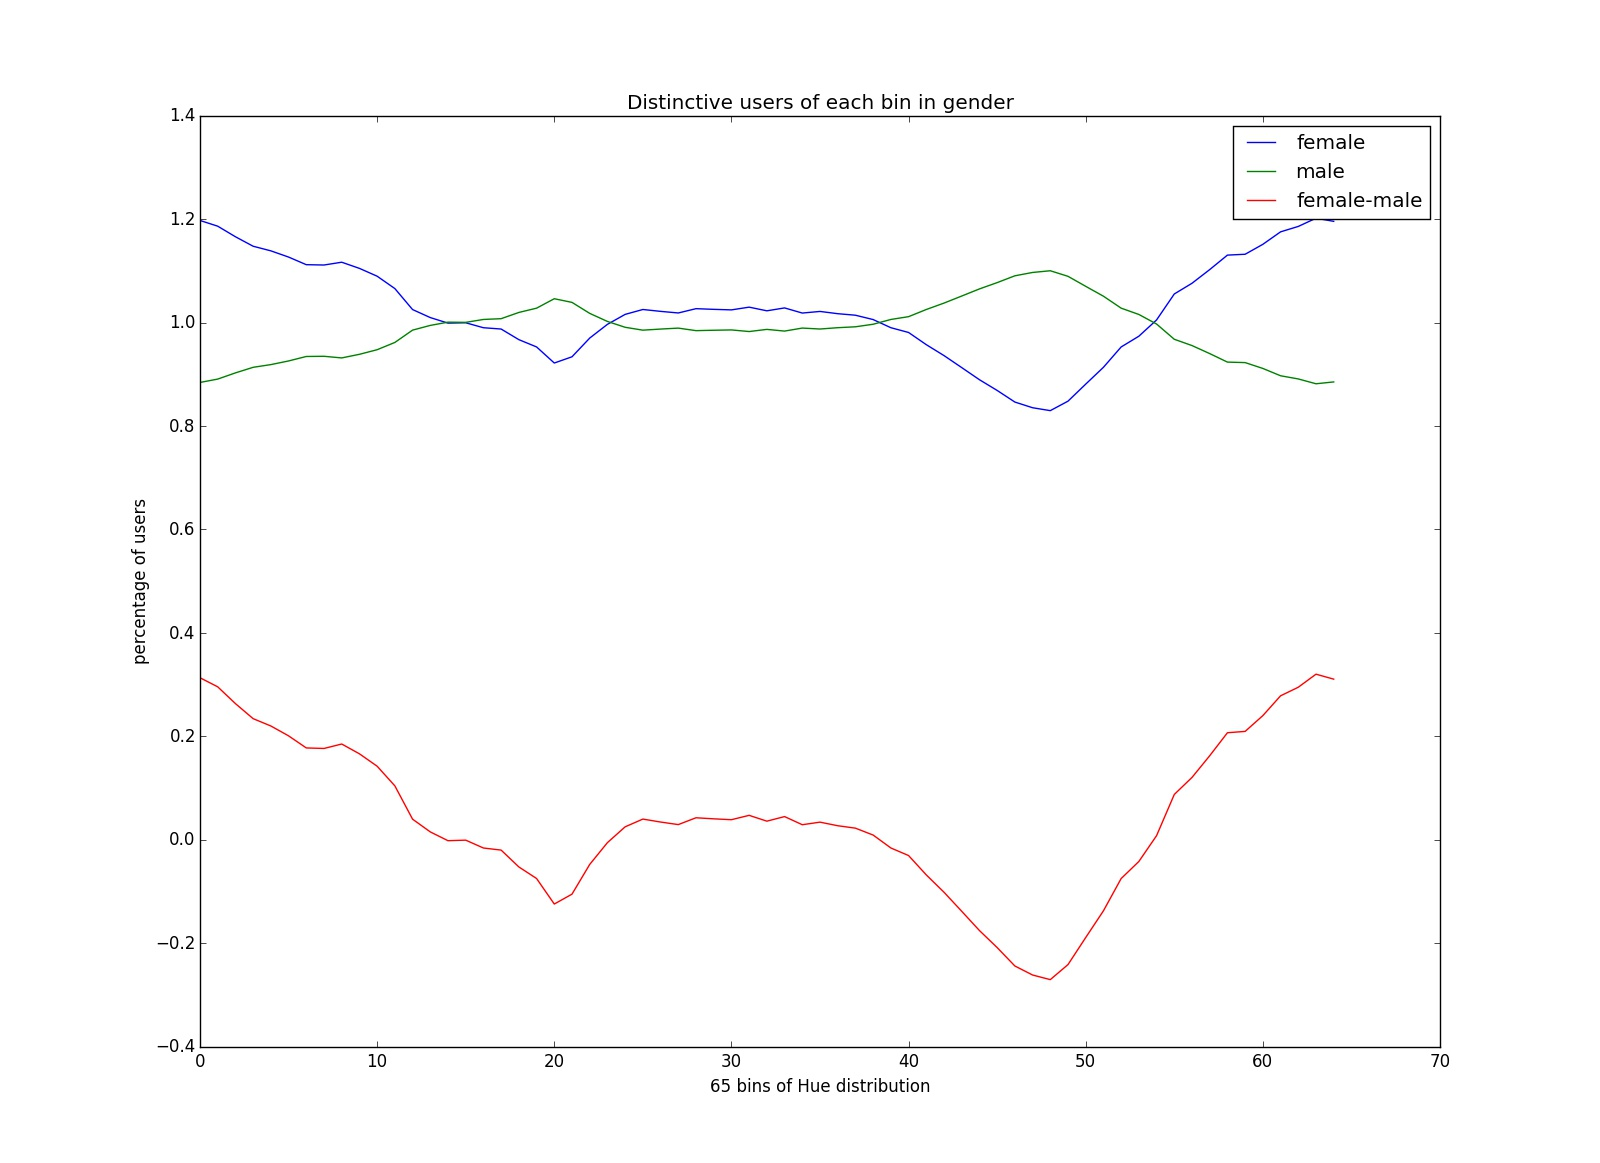
\includegraphics[width=0.489\textwidth]{figures/chapter3/topusergender.jpeg}
 \caption{Number of users with more than $10\%$ color pixels in each color bin (according to Allpeople dataset) showing the consistaent result of gender preference on redish and bluish color.}
 \label{fig:user}
\end{figure}

\section{Genders Preference on Contents}

To give a general idea of what content people take pictures of when they prefer certain colors, we perform a further experiment. Generally people would like to tag their images with the occasion, names of people in the picture and their most interested objects. Therefore, we consider the image tags to represent the content of images.

We rank all the tags appearing in 15 million images in the Random dataset, normalized by users, to find the 500 most frequently used tags. To better visualize the tag distribution, we adopt the hue space of Palmer 32 colors~\cite{palmer32color}. 
These are 32 evenly-speed color points in LCh space, including eight hues in each of two lightness and two chroma values (giving Light, Muted, Dark, and Saturated variants of each hue).

We find images containing more than $10\%$ pixels of each of the 8 hues.
In these images, we aggregate them to users. So each tag used multiple times in images from one user, is only counted once. 
In this way, we compute the tag frequency and entropy across 8 hue centers, for all users, and for male and female users respectively.
We compose the tag distribution maps in two ways.
Firstly, for each hue, find the top 10 most frequently used tags and sort them by the least entropy, presented in Fig. ~\ref{fig:tag} with female user tags on top, male users in the middle and all users at the bottom.
In the second way, the top 500 tags are sorted by entropy value first. Along this list, we find 10 most frequently used tags for each hue. This plot is also presented in Fig. ~\ref{fig:tag} in the same way as the first plot.

\begin{figure*}[th]
\centering
\begin{tabular}{c}
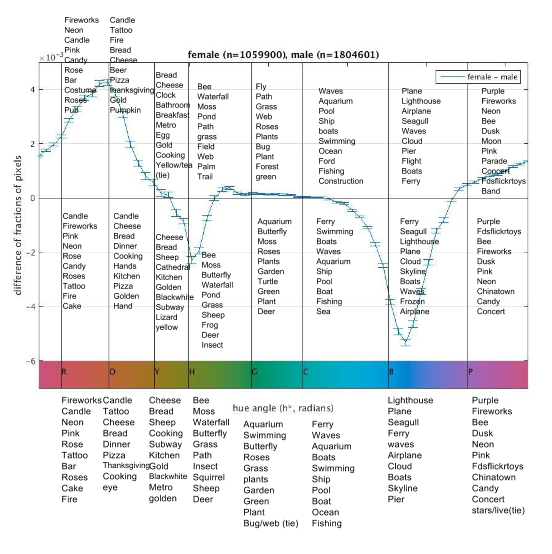
\includegraphics[width=0.65\textwidth]{figures/chapter3/tag1.png} \\
(a) Frequency tag distribution sorted by entropy ascendingly.\\
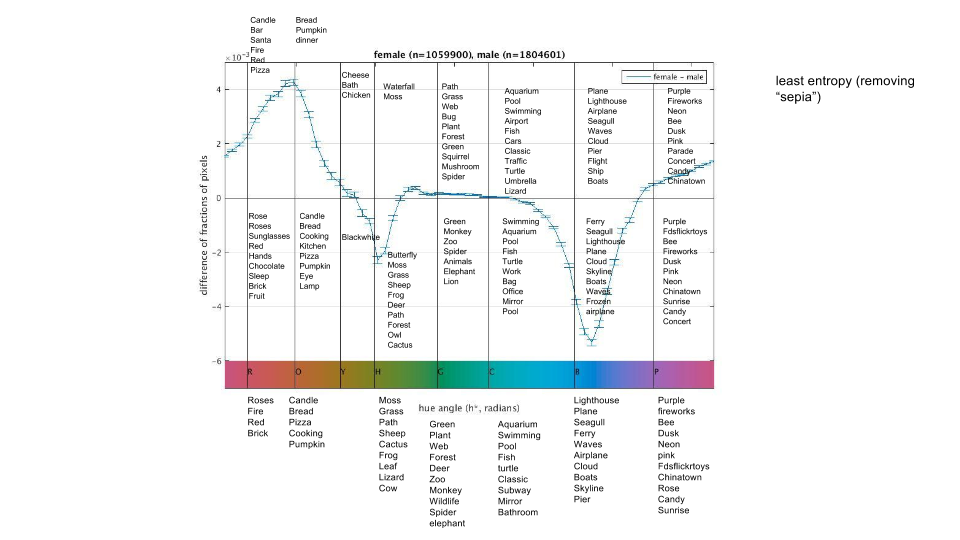
\includegraphics[width=0.65\textwidth]{figures/chapter3/tag2.png} \\
(b) Frequency tag distribution sorted by overall tag entropy.\\
\end{tabular}
\caption{Most concentrated tags on each Palmer color hue for female and male users.}
\label{fig:tag}
\end{figure*}





\section{Color Distribution of Flickr vs. Street View}
The next research question we address is the difference between Flickr photos and the environment where the photographers could have taken pictures. 
We plot the color distribution in histogram of Palmer 32 colors.

To estimate color distributions in the environment, we collect data from Google Street View.
For each geotagged Flickr photo, we query the Google Street View Image API with its GPS information, and download Street View images in 4 view angles (0, 90, 180, 270 degree). If there are no Street View images available for a GPS location, we discard the corresponding Flickr photo.

The result turns out to be very interesting in respect to locations. In Fig. ~\ref{fig:street}, we present the results of three locations of Death Valley National Park, Disneyland at Los Angeles and San Diego Balboa Park. 
In general, we observe the preference of saturated color and reddish color of human compared to the environment.

\begin{figure*}
\centering
\begin{tabular}{m{0.6\linewidth}}
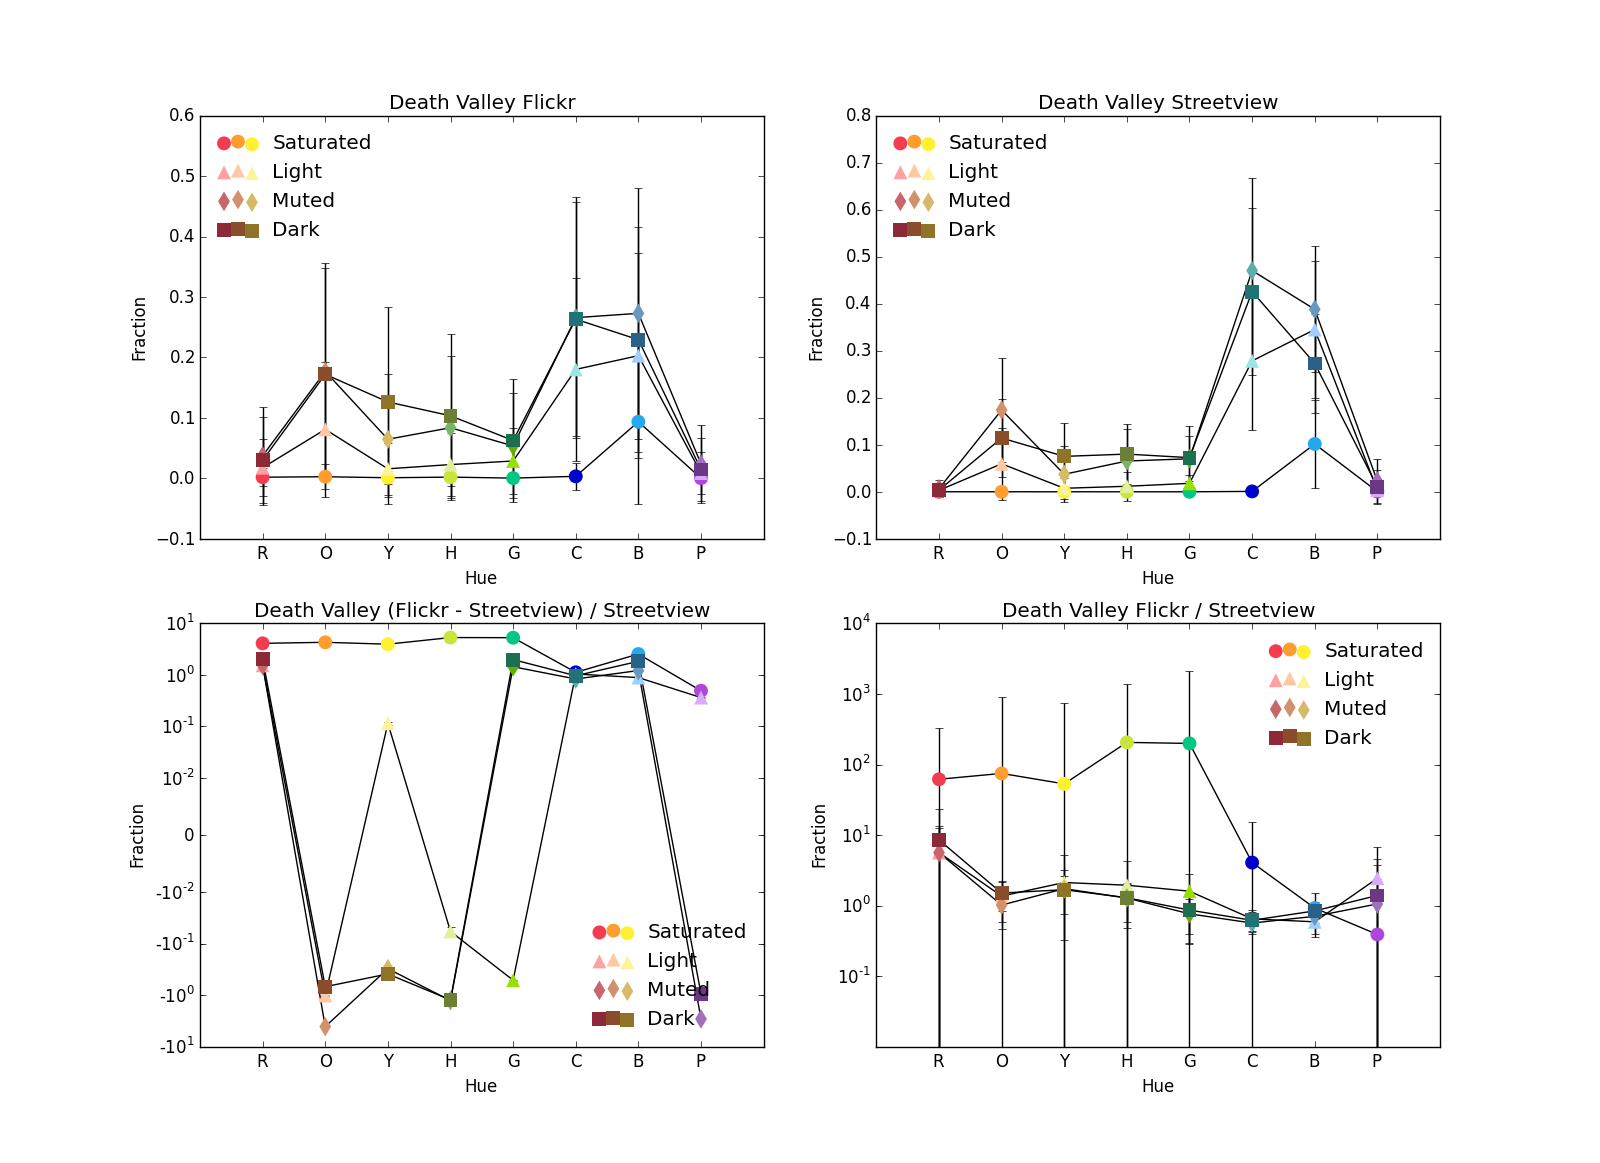
\includegraphics[width=0.55\textwidth]{figures/chapter3/deathvalleyflkstr.png} \\
(a) Deathvalley National Park. It shows photographers prefer warm color in general.\\
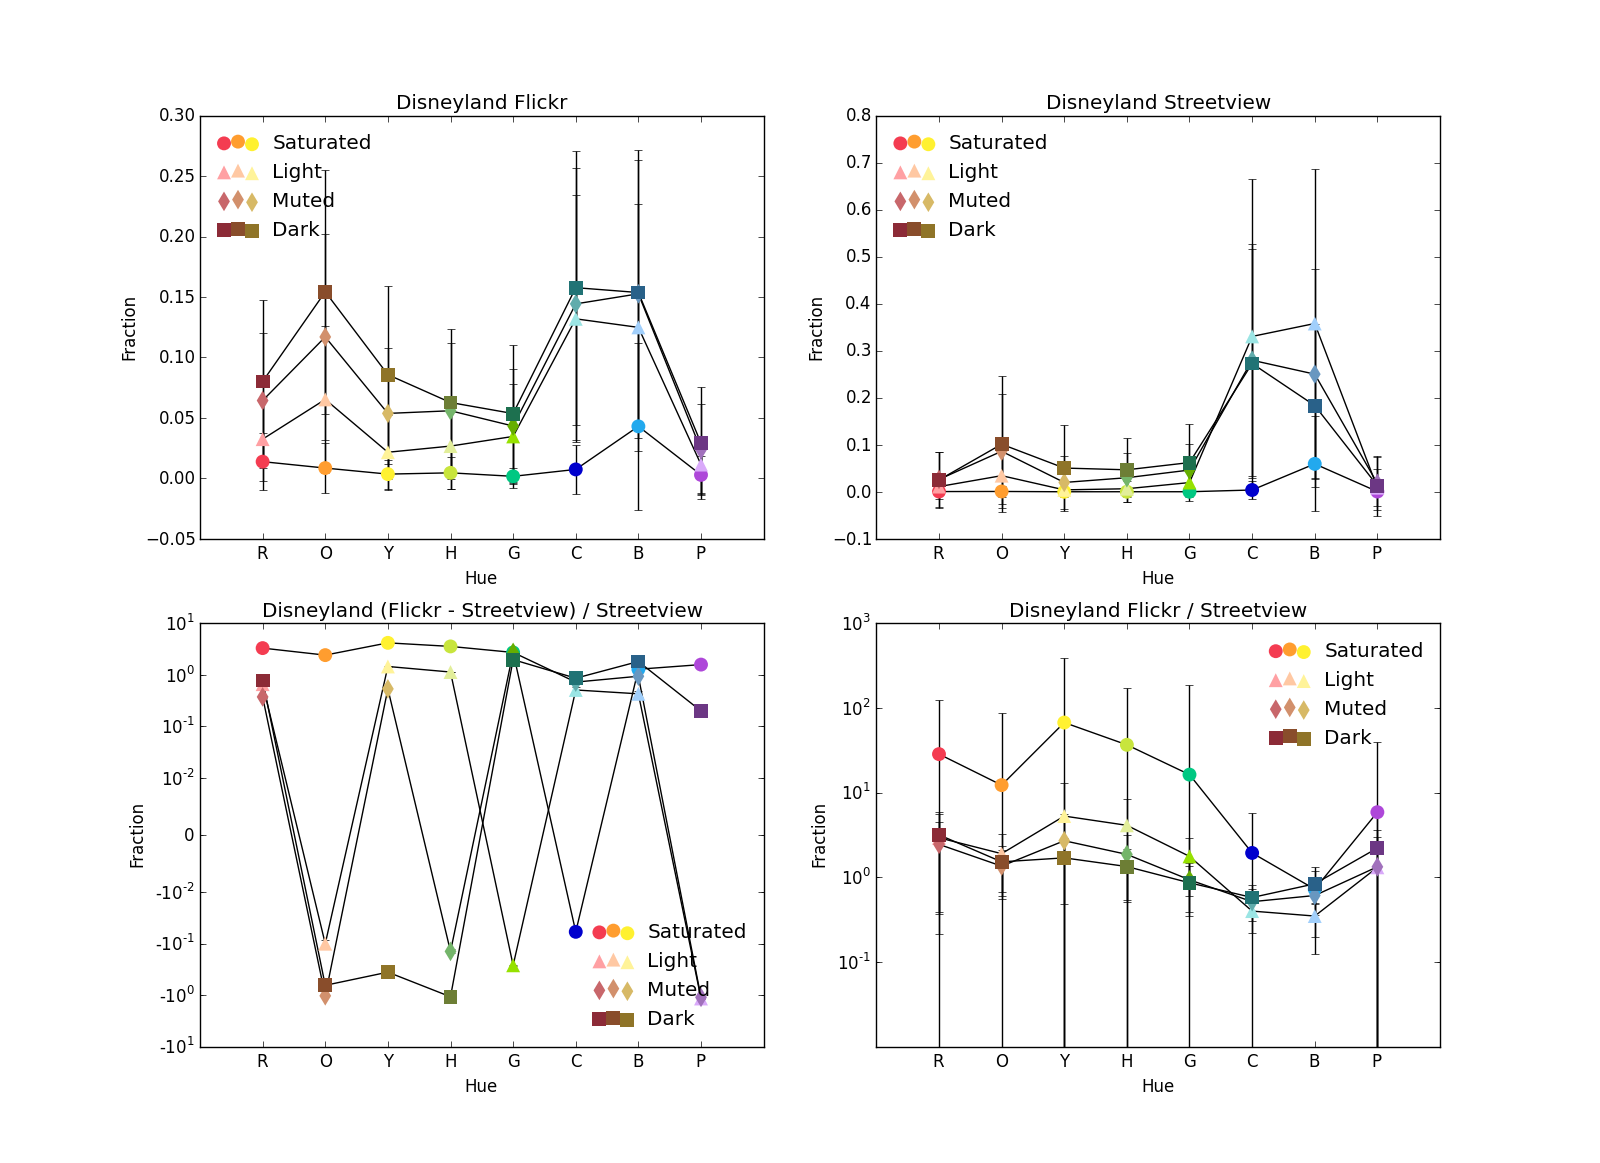
\includegraphics[width=0.55\textwidth]{figures/chapter3/disneyflkstr.png} \\
(b) DisneyLand at Los Angeles. There is more warm color and more saturated color to see in Disneyland so that we see a clearer preference of the photographers.\\
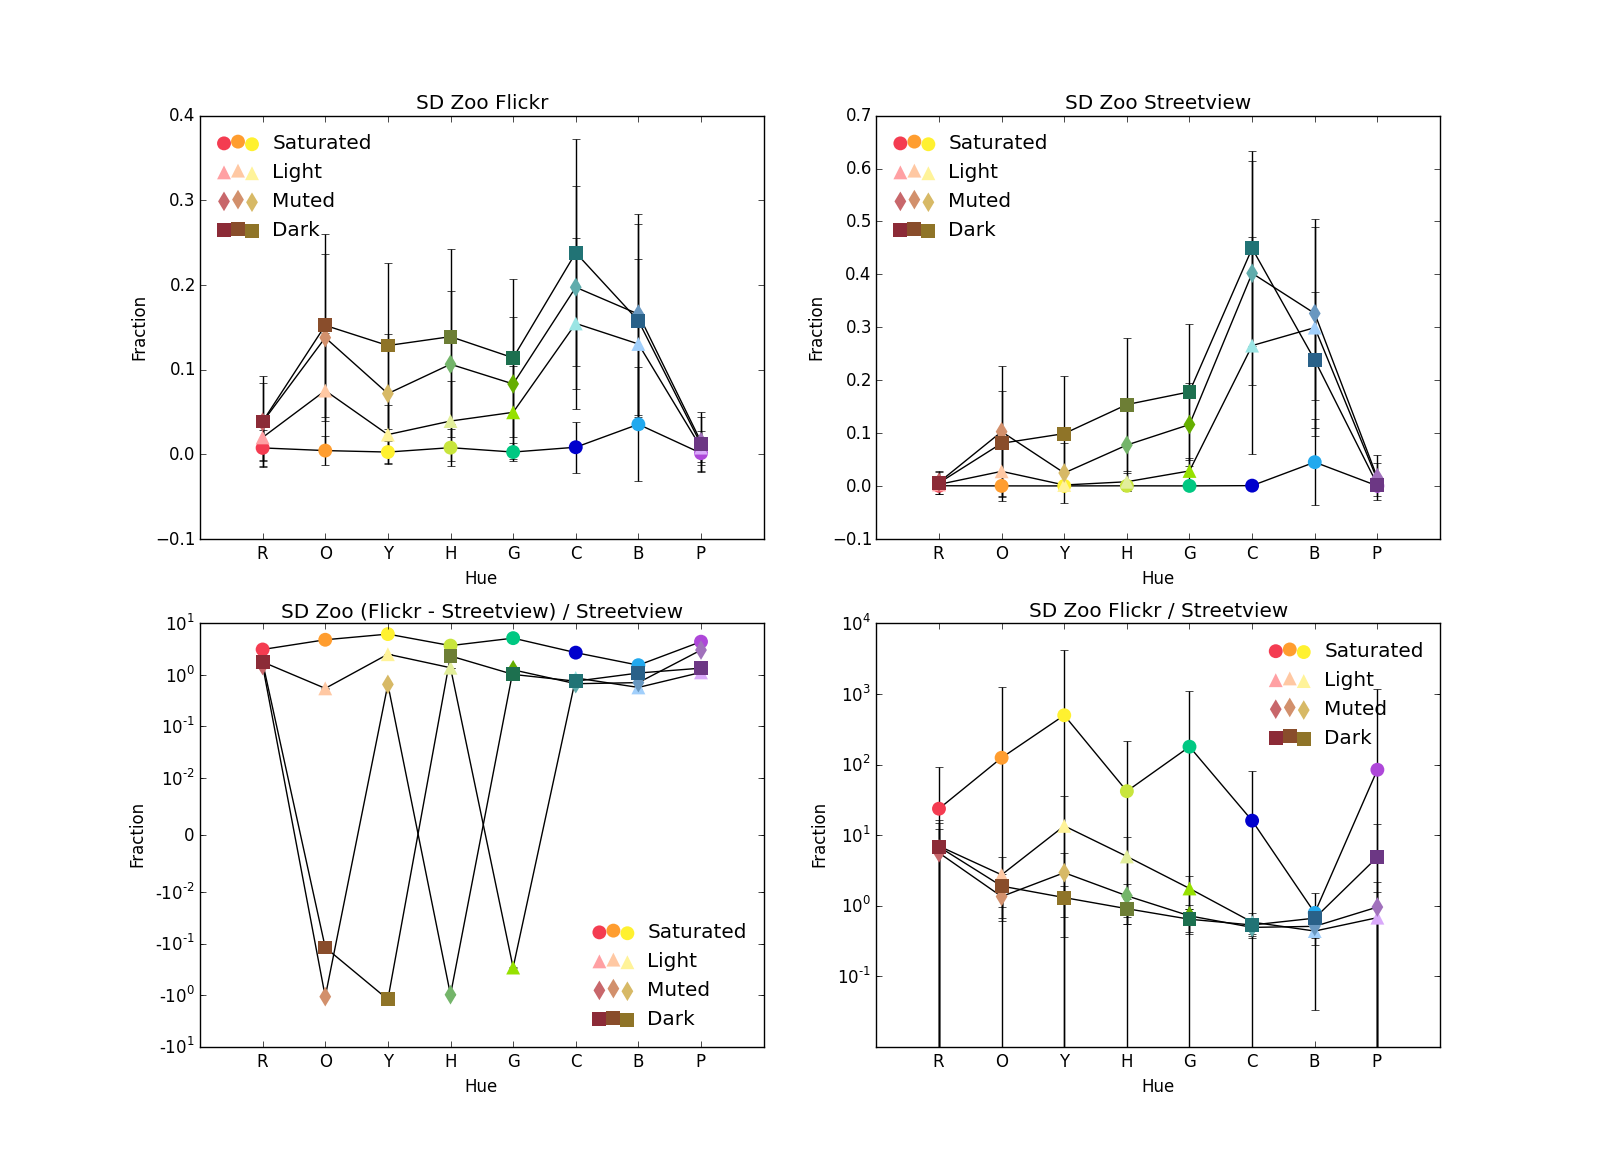
\includegraphics[width=0.55\textwidth]{figures/chapter3/sdzooflkstr.png} \\
(c) San Diego Balboa Park. In this very green place, we observe that people do not show as much interest in greenish objects.\\
\end{tabular}
\caption{Comparison of hue distribution in Palmer's 32 colors for flickr photos and the Google Street View images at the same GPS lcoation.}
\label{fig:street}
\end{figure*}

